% !TeX encoding = UTF-8
% !TeX spellcheck = es_ES
% Chapter 1

\newcolumntype{L}[1]{>{\raggedright\let\newline\\\arraybackslash\hspace{0pt}}m{#1}}
\newcolumntype{C}[1]{>{\centering\let\newline\\\arraybackslash\hspace{0pt}}m{#1}}
\newcolumntype{R}[1]{>{\raggedleft\let\newline\\\arraybackslash\hspace{0pt}}m{#1}}

\chapter{Introducción General} % Main chapter title

\label{Chapter1}
\label{IntroGeneral}

En el presente capítulo se presentan brevemente diferentes equipos para control de accesos, las tecnologías de identificación utilizadas por los mismos, los motivos que condujeron al desarrollo del trabajo junto con los objetivos y alcances del mismo.

\section{Descripción del problema}
\label{sec:descripcion}

El control de las personas que acceden a un ambiente es una de las aplicaciones que más se beneficiaron con los avances de la electrónica. El cambio de las cerraduras mecánicas, y sus correspondientes llaves, por sistemas electrónicos lleva más de 30 años y continúa en plena expansión. Actualmente existe en el mercado una oferta muy amplia y variada de equipos, que utilizan diferente medios para identificar a las personas que intentan acceder. Los métodos de identificación más difundidos en la actualidad son:

\begin{itemize}
	\item Clave numérica: para la identificación de cada usuario se le asigna una clave numérica que se debe ingresar mediante un teclado que forma parte del equipo. Este esquema es el más económico pero también el más inseguro, ya que la clave puede fácilmente darse a conocer a personas no autorizadas. 
	\item Tarjetas de proximidad: para la identificación del portador se utilizan unos sistemas electrónicos que se alimentan al aproximarlos a un lector y transmiten información. Las tarjetas en realidad pueden adoptar otros formatos como llaveros o etiquetas autoadhesivas. Este esquema resulta más costoso pero también más seguro que el anterior ya que las tarjetas no pueden replicarse fácilmente, aunque sí es posible prestarlas a personas no autorizadas.
	\item Reconocimiento de huella digital: para la identificación se toma una imagen de un dedo del usuario y se reconoce la geometría de las huellas digitales. Este esquema es el más costos y seguro de todos, ya que duplicar una huella digital es una tarea realmente compleja.
\end{itemize}

Independientemente del medio utilizado para la identificación del usuario, todos los equipos tienen una forma de operación y configuración similar, la que puede ser clasificada en tres grandes grupos:

\begin{itemize}
	\item Equipos autónomos: son los más económicos y fáciles de instalar, ya que solo requieren alimentación y la conexión con el mecanismo que libera la puerta para permitir el acceso. Dentro de este grupo podemos encontrar incluso equipos que se integran dentro de una cerradura tradicional y se alimentan con baterías, lo que simplifica al máximo su instalación. La principal desventaja de este tipo de equipos es la gestión de las personas autorizadas a ingresar. En general estos equipos integran unos teclados muy básicos con los que se pueden agregar y borrar las personas autorizadas mediante secuencias de códigos numéricos bastante poco amigables con los usuarios finales.
	\item Equipos en línea: son los más seguros pero también los más costos y complejos de instalar. Estos equipos incorporan una interfaz de comunicaciones para validar cada operación de acceso con un servidor central en tiempo real. De esta forma, la gestión de las personas autorizadas se realiza en forma centralizada sobre dicho servidor mediante un programa informático mucho más simple de utilizar. Este esquema puede, además, incorporar mayor complejidad en las validaciones efectuadas para autorizar el ingreso de una persona. La principal desventaja de este esquema es que resulta muy sensible a una falla en la red de comunicaciones o en el servidor de autorizaciones.
	\item Equipos gestionados: son equipos autónomos que incorporan una interfaz de comunicaciones para permitir su gestión en una forma más simple. En muchos casos son equipos que pueden además operar en línea. Podría pensarse que estos equipo combinan las desventajas de los dos anteriores, pero esto no es verdad. Si bien el costo es mayor que el de un equipo autónomo,  no requiere toda la infraestructura de los equipos que operan en línea, lo que disminuye significativamente el costo total de la solución. A cambio de ese aumento en el costo permiten una gestión más simple, ya que es posible utilizar una computadora con un software amigable.
\end{itemize}

Como se desprende del análisis anterior, resulta muy difícil encontrar un equipo adecuado para el mercado hogareño o de pequeñas oficinas. A pesar de que la oferta del mercado es muy amplia, no existen muchos equipos que combinen adecuadamente las características de precio con la facilidad de instalación y gestión necesarias en un ambiente donde el usuario final posee conocimientos técnicos muy limitados. Por estas razones la mayoría de los equipos destinados a este mercado corresponden al grupo de los equipos gestionados. Sin embargo, la mayoría de ellos utilizan interfaces de comunicaciones cableadas, las que complican la instalación y permiten la gestión únicamente desde una computadora.

\section{Motivación}
\label{sec:motivacion}

Punku nace como una propuesta de la firma EQUISER para resolver el problema del control de accesos en hogares, pequeñas oficinas, consorcios de departamentos y cocheras\cite{equiser_sistema_nodate}. Las características más importantes de este mercado son la poca cantidad de puertas controladas, falta de personal técnico para la gestión del equipo, y en el caso de los consorcios y cocheras, frecuentes cambios en la lista de personas autorizadas. Para lograr la mejor relación entre seguridad, precio y facilidad de gestión, el equipo puede funcionar con tarjetas de proximidad o con controles remotos. Además utiliza una interfaz Bluetooth que permite gestionarlo desde un dispositivo móvil, ya sea una computadora portátil, un teléfono celular inteligente o una tableta. También incorpora una entrada para un sensor que permite detectar la apertura de la puerta, y una salida de alarma para informar cuando permanece abierta más tiempo del especificado. 

En la figura \ref{fig:BloquesActual} se presenta el diagrama de bloques del equipo, donde se pueden observar dos unidades funcionales:

\begin{figure}[ht]
	\centering
	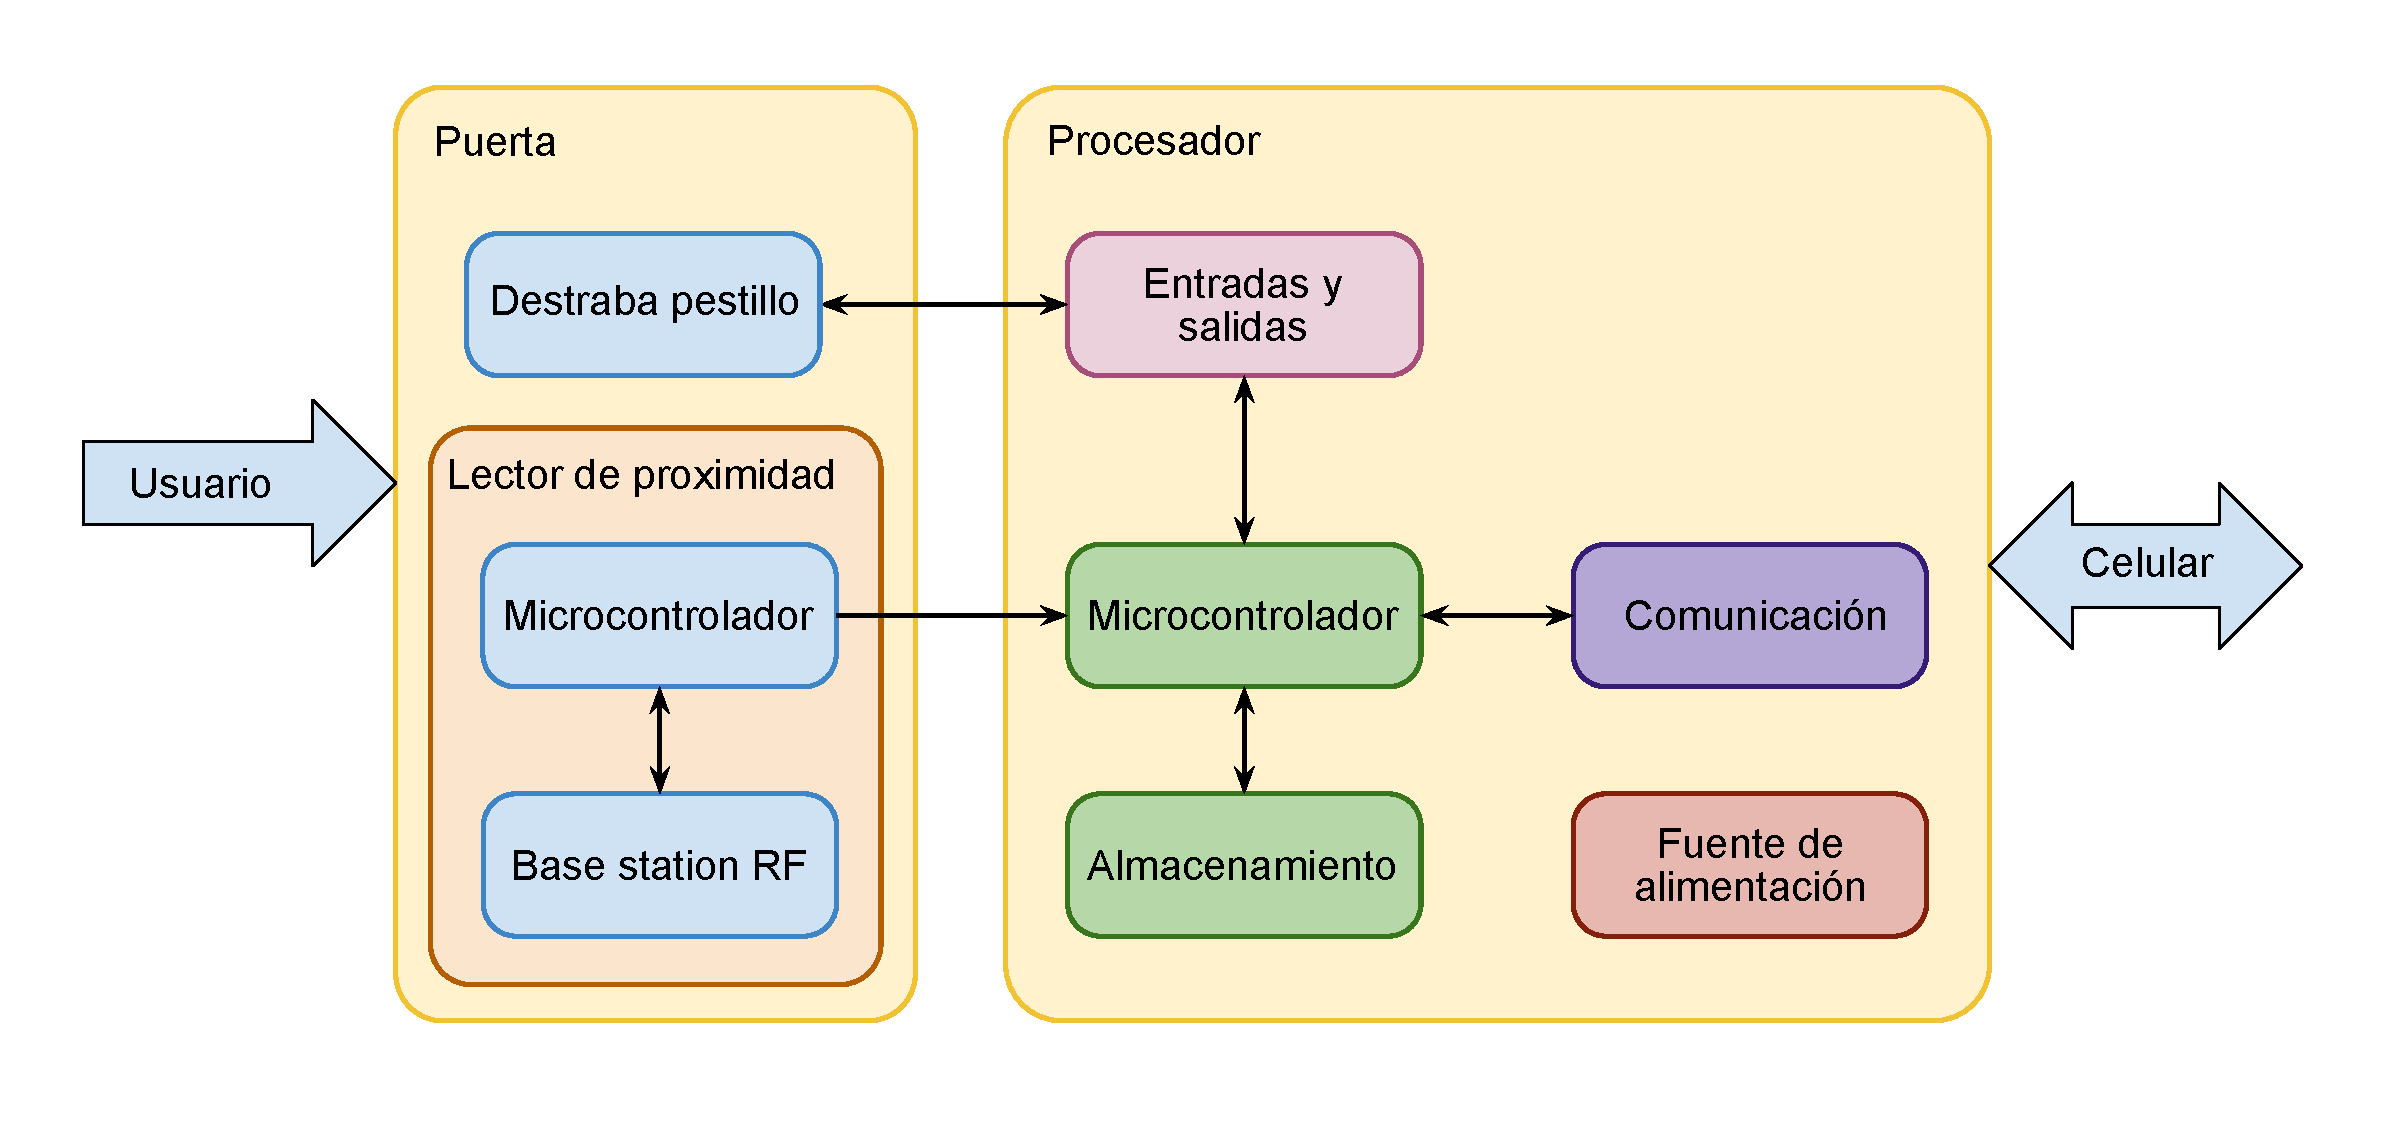
\includegraphics[width=\textwidth]{./Figures/BloquesActual.pdf}
	\caption{Diagrama de bloques del equipo actual}
	\label{fig:BloquesActual}
\end{figure}

\begin{itemize}
	\item La lectora de proximidad: es la responsable de generar el campo magnético que alimenta a las tarjetas y decodificar la información enviada por estas.
	\item El procesador: es el responsable de determinar si la tarjeta leída puede o no acceder, registrar los movimientos de acceso, accionar las salidas para autorizar el ingreso, supervisar el estado de la puerta y comunicarse con el equipo móvil para permitir gestionar su configuración.
\end{itemize}

Como puede notarse en figura \ref{fig:EquipoActual}, donde puede ver una imagen del equipo actual, cada una de estas unidades funcionales se encuentra alojada en un gabinete independiente. De esta manera la lectora de proximidad se puede instalar del lado externo de la puerta y el procesador del lado interno, evitando la manipulación del cableado para forzar la apertura de la puerta.

\begin{figure}[ht]
	\centering
	\vspace{3mm}
	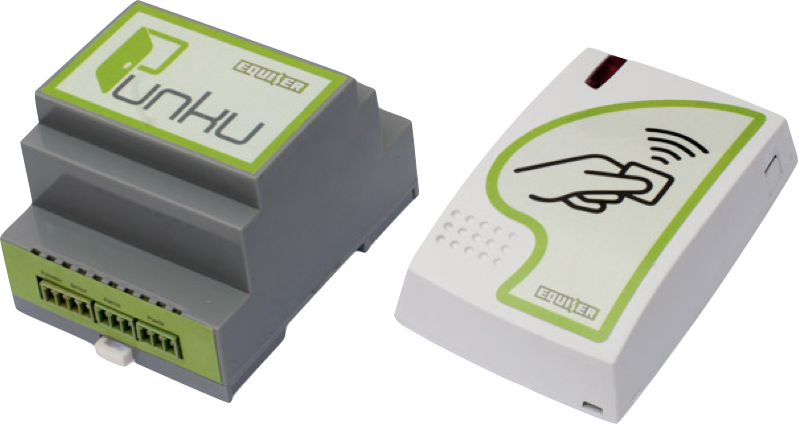
\includegraphics[scale=.5]{./Figures/EquipoActual.png}
	\caption{Fotografía del equipo actual}
	\label{fig:EquipoActual}
\end{figure}

En la tabla \ref{tab:ComparacionActual} se puede ver un cuadro comparativo del producto actual con otros equipos existentes en el mercado. Como se puede observar, la oferta se polariza en dos tipos de equipos: totalmente autónomos gestionados mediante un teclado numérico muy limitado o equipos con conexiones cableadas (ethernet o usb) que solo pueden ser gestionados desde computadoras de escritorio o portátiles. En el mercado internacional sí existen equipos que se pueden gestionar desde un dispositivo móvil, pero tampoco en este escenario la oferta es abundante. Por estas razones Punku constituye una solución atractiva que busca imponerse en el mercado principalmente gracias a la facilidad de manejo por parte del usuario final. 

\begin{table}[ht]
	\centering
	\caption{Cuadro comparativo con otros equipos del mercado}
	\begin{tabular}{C{25mm} C{25mm} C{50mm} C{20mm}}    
		\toprule
		\textbf{Equipo}  
			& \textbf{Tecnología} 
			& \textbf{Forma de gestión}
			& \textbf{Valor}  \\
		\midrule
		EQUISER \newline Punku 
			& Proximidad y remotos RF
			& Gestionado desde un \newline celular usando Bluetooth
			& \$ 15.000\\
		\midrule
		Tebas \newline 208NW \cite{noauthor_control_nodate}
			& Proximidad
			& Teclado numérico \newline integrado en el equipo
			& \$ 4.000\\
		\midrule
		ZK \newline MA300IS \cite{noauthor_control_nodate-2}
			& Proximidad \newline y huellas
			& Computadora conectada \newline mediante Ethernet
			& \$ 10.000\\
		\midrule
		ANVIZ \newline T5 Pro \cite{noauthor_control_nodate-1}
			& Proximidad \newline y huellas
			& Computadora conectada \newline mediante Ethernet o USB
			& \$ 8.000\\
		\bottomrule
		\hline
	\end{tabular}
	\label{tab:ComparacionActual}
\end{table}

La versión de Punku que se produce actualmente cubre adecuadamente las necesidades del mercado al cual está destinado. Sin embargo el diseño del equipo se remonta al año 2013, y los cambios en las tecnologías sumados a nuevas posibilidades de uso demandaban una actualización. Después de un análisis de las fortalezas y debilidades del equipo se determinó que era necesario realizar las siguientes mejoras:  

\begin{itemize}
	\item Cambio del procesador principal: para el desarrollo original se utilizó un microcontrolador producido por la empresa Freescale, perteneciente la familia \emph{ColdFire}\cite{noauthor_nxp_2019}. Con el avance de los procesadores \emph{Cortex} el fabricante fue dejando de lado el desarrollo de esta gama de productos, por lo que en este momento el microcontrolador utilizado resulta más costoso que un procesador más nuevo con mayores prestaciones. Lamentablemente no existe una oferta por parte del fabricante de un microcontrolador con una disposición de terminales pensada para efectuar un reemplazo directo del utilizado actualmente.
	
	\item Cambio de la interfaz de comunicaciones: el equipo actual utiliza para la comunicación una interfaz Bluetooth 2. Poco tiempo después del desarrollo se aprobó la versión 4 de este protocolo, la que fue rápidamente adoptado por la firma Apple. Esta nueva versión del protocolo no es compatible con la anterior, y si bien algunos equipos pueden funcionar en ambos modos de trabajo, este no es el caso de los equipos \emph{iPhone}, donde para privilegiar la duración de la batería solo pueden operar con Bluetooth 4.
	
	\item Incorporación de un reloj: al comercializar las primeras unidades surgió el requerimiento de algunos clientes para disponer de un registro de acceso con fecha y hora de cada evento. El equipo actual no dispone de un RTC (\emph{Real Time Clock}) que le permita mantener la fecha y hora cuando no dispone de alimentación eléctrica. De esta forma, si bien el equipo registra los eventos con fecha y hora, se vuelve a una fecha inicial preestablecida cada vez que se reinicia, y es necesaria una comunicación desde el celular para reajustar el reloj interno. El resultado es que la mayoría de los registros de accesos no tienen una fecha y hora válidas.
	
	\item Soporte para cerraduras motorizadas: uno de los principales obstáculos en la instalación de equipos para el control de accesos en el mercado al cual está destinado Punku, son los cortes de alimentación eléctrica. Según el tipo de cerradura que se utilice, ante una falla de energía la puerta quedará cerrada y no se podrá acceder, o peor aún, quedará abierta en forma permanente. Una solución a este problema es combinar una cerradura con llave y un sistema motorizado que permita la liberación y el bloqueo de la puerta por cualquiera de los medios. Para esto el equipo debe poder invertir la alimentación en la salida que controla al motor, y de esta forma liberar o bloquear el mecanismo en función del sentido de giro de este.
	
	\item Gestión desde la nube: con el avance en la conectividad a Internet se volvió más común disponer de equipos que pueden ser gestionados en forma remota. En el caso de un control de accesos siempre resulta atractiva la posibilidad de cambiar el permiso de acceso de una persona en forma inmediata sin necesidad de estar cerca del equipo. El uso de Bluetooth como interfaz de comunicaciones resulta un obstáculo para esta funcionalidad por su corto alcance y porque nunca se popularizaron equipos equivalentes a los \emph{routers} de WiFi que permitan el acceso a Internet utilizando Bluetooth.
\end{itemize}

\section{Objetivos y alcance}
\label{sec:objetivos}

El objetivo general del trabajo desarrollado fue el diseño y la implementación del prototipo de una nueva versión del equipo para control de accesos Punku que resolviera los problemas mencionados en la sección \ref{sec:motivacion}. 

Los objetivos particulares definidos para este fueron:

\begin{enumerate}
	\item Diseñar el nuevo equipo utilizando un módulo de la familia ESP32 \cite{noauthor_esp32_2019} del fabricante Espressif, el cual incorpora interfaces de comunicación WiFi y Bluetooth en las versiones 2 y 4.
	
	\item Agregar al nuevo equipo un circuito integrado RTC con respaldo de batería que le permita mantener la fecha y hora válidas, aun cuando se produzcan interrupciones en el suministro de energía eléctrica.
	
	\item Agregar al nuevo equipo la posibilidad de invertir la polaridad de alimentación en la salida que libera la cerradura de forma tal que se pueda utilizar un sistema motorizado para destrabar la puerta.
	
	\item Mantener las características generales del equipo actual en el nuevo diseño, tratando en lo posible de mejorar aún más la facilidad de gestión del equipo y de disminuir su costo.
	
	\item Desarrollar el firmware del equipo desde cero, utilizando un sistema operativo de tiempo real y un diseño modular que permita escalar las funcionalidades del equipo.
\end{enumerate}

El resultado esperado es entonces un prototipo totalmente funcional, que incorpore las mejoras ya mencionadas, acompañado de la siguiente documentación:

\begin{enumerate}
	\item Diagrama esquemático del equipo en el programa KiCad.
	\item Diseño de la placa electrónica realizada en el programa KiCad.
	\item Especificación de requisitos del firmware según el estándar IEEE-830.
	\item Arquitectura y el diseño detallado del firmware modelado utilizando diagramas UML.
	\item Pruebas de aceptación para validar el correcto funcionamiento del equipo escritas en metalenguaje Gherkin. 
	\item Código fuente del firmware para el control del equipo con documentación y comentarios adecuados que faciliten su compresión.
\end{enumerate}